\section{Architecture overview}
\label{app:arch}
Figure~\ref{fig:arch} contrasts baseline NCM and APC-NCM.

\begin{figure*}[t]
\centering
\begin{tikzpicture}[font=\footnotesize, node distance=4mm and 6mm,
 box/.style={draw, rounded corners=2pt, minimum height=6mm, align=center, fill=white},
 gen/.style={box, fill=blue!8}, cor/.style={box, fill=orange!18}, dec/.style={box, fill=green!10}, hal/.style={box, fill=red!8, diamond, aspect=2.2, inner sep=1pt},
 >={Stealth[length=2mm]}]
\node[font=\bfseries\footnotesize] (tA) at (0,0.9) {(a) Baseline NCM};
\node[gen] (g0) at (0,0) {$G_\phi$\\level $k$};
\node[box, right=of g0] (p0) {$\zh^{(k)}=\zh^{(k-1)}$\\$+\Phi_k\Up_k E_k(\hat r_k)$};
\node[box, right=of p0] (d0) {$\mathrm{Down}_{k+1}$};
\node[gen, right=of d0] (g1) {$G_\phi$\\level $k{+}1$};
\node[dec, right=12mm of g1] (o0) {$D_\psi(\zh^{(K-1)})$\\after all $K$ levels};
\draw[->] (g0) -- node[above]{$\hat r_k$} (p0); \draw[->] (p0) -- (d0); \draw[->] (d0) -- node[above]{$u_{k+1}$} (g1); \draw[->, dashed] (g1) -- node[above]{$\cdots$} (o0);
\node[font=\bfseries\footnotesize] (tB) at (0,-1.35) {(b) APC-NCM};
\node[gen] (G0) at (0,-2.3) {$G_\phi$\\level $k$};
\node[box, right=of G0] (P0) {predictor\\ \eqref{eq:pred}};
\node[cor, right=of P0] (C0) {corrector $C_\omega$\\ \eqref{eq:corr}};
\node[hal, right=of C0] (H0) {$\Delta_k{<}\tau$?};
\node[box, right=of H0] (D0) {$\mathrm{Down}_{k+1}$};
\node[gen, right=of D0] (G1) {$G_\phi$\\level $k{+}1$};
\node[dec, below=6mm of H0] (O0) {$D_\psi(\zt^{(k^\ast)})$};
\node[box, above=3mm of C0, fill=gray!10] (pf) {$h_{\mathrm{prefix}}$, level $k$};
\draw[->] (G0) -- node[above]{$\hat r_k$} (P0); \draw[->] (P0) -- node[above]{$\zh^{(k)}_{\mathrm{pred}}$} (C0); \draw[->] (C0) -- node[above]{$\zt^{(k)}$} (H0);
\draw[->] (H0) -- node[above]{no} (D0); \draw[->] (D0) -- (G1); \draw[->] (H0) -- node[right]{yes: halt} (O0); \draw[->] (pf) -- (C0);
\draw[->, densely dotted, orange!70!black] (P0.south) to[out=-40,in=-140] node[below=9mm, pos=0.5, font=\scriptsize, text=orange!70!black]{decode-path variant: $u_{k+1}$ bypasses $C_\omega$} (D0.south);
\end{tikzpicture}
\caption{Baseline NCM (a) adds one quantized residual per level and always runs all $K$ levels. APC-NCM (b) revises the cumulative latent with a learned corrector and may halt once the latent flux (or decoder instability) falls below $\tau$. In the in-loop variant the corrected latent feeds the next generator level; in the decode-path variant (dotted) the generator continues from the uncorrected latent and $C_\omega$ acts only on decoded latents.}
\label{fig:arch}
\end{figure*}

\section{Algorithm}
\label{app:alg}
Algorithm~\ref{alg:apc} summarizes training and inference.

\begin{algorithm}[t]
\caption{APC-NCM training and inference}
\label{alg:apc}
\begin{algorithmic}[1]
\Require frozen $E_\theta,D_\psi,\{\mathcal{V}_k,\Phi_k\}$, $G_\phi$; training inputs/references $\{(c_i,y_i)\}_{i\le N_{\mathrm{tr}}}$
\State \textbf{Training}
\For{$i=1,\dots,N_{\mathrm{tr}}$}
  \State $(\zh^{(k)}_{\mathrm{GT}})_k\gets$ \texttt{z\_to\_idx}$(E_\theta(y_i))$;\quad $(\zh^{(k)}_{\mathrm{roll}})_k\gets$ greedy rollout of $G_\phi$ on $c_i$
  \State $(\zh^{(k)}_{\mathrm{cor}})_k\gets$ cumulative latents of codes corrupted at rate $u\sim\mathcal{U}(0,1)$, level 0 kept
\EndFor
\State minimize~\eqref{eq:loss} with AdamW, one-cycle LR; keep best validation epoch (identity included)
\State choose $s$ (or $s_k$) by closed-loop validation quality; choose rule and $\tau$ on $\{c_i\}$
\State \textbf{Inference} on a batch of prefixes $c$
\State $\zh^{(-1)}\gets 0$; sample $\hat r_0$ with $G_\phi$
\For{$k=0,\dots,K-2$}
  \State $\zh^{(k)}\gets\zh^{(k-1)}+\Phi_k\Up_kE_k(\hat r_k)$ \Comment{predictor}
  \State $\zt^{(k)}\gets\zh^{(k)}-\eta_kC_\omega(\zh^{(k)},h_{\mathrm{prefix}},k)$ \Comment{corrector}
  \If{freezing} copy rows of $\zh^{(k-1)}$ into frozen segments \EndIf
  \If{$k\ge k_{\min}$ \textbf{and} halting criterion holds for all sequences} \Return $D_\psi(\zt^{(k)})$ \EndIf
  \State $u_{k+1}\gets\mathrm{Down}_{k+1}(\zt^{(k)})$ (in-loop) or $\mathrm{Down}_{k+1}(\zh^{(k)})$ (decode-path)
  \State $\hat r_{k+1}\gets\argmax G_\phi(u_{k+1},c)$
\EndFor
\State \Return $D_\psi\big(\zh^{(K-2)}{+}\Phi_{K-1}E_{K-1}(\hat r_{K-1})\big)$, corrected at level $K{-}1$ in the decode-path variant
\end{algorithmic}
\end{algorithm}

\section{Hardware, profiling and hyper-parameters}
\label{app:hw}
\textbf{Hardware and profiling.} Every number comes from Kaggle Tesla T4 (16\,GB, 14.6\,GB usable) sessions with Python 3.13 and the preinstalled PyTorch~\citep{paszke2019pytorch} CUDA build. Wall-clock latency is the mean over evaluation batches after one untimed warm-up batch, synchronized with \texttt{torch.cuda.synchronize}; peak memory is \texttt{torch.cuda.max\_memory\_allocated}. Variants of the same task were timed in the same session. Hyper-parameters are listed in Table~\ref{tab:hp}.

\begin{table}[t]
\centering
\caption{Hyper-parameters. Generator and tokenizer settings are those of the official evaluation configs.}
\label{tab:hp}
\footnotesize\setlength{\tabcolsep}{2.5pt}
\begin{tabular}{lccc}
\toprule
 & Sudoku & WMT14 & XSum\\
\midrule
levels $K$ & 12 & 11 & 9\\
$L$, $d$ & 89, 256 & 64, 768 & 48, 768\\
generator params & 25.5M & 120.0M & 88.0M\\
$C_\omega$ params (width) & 1.23M & 1.20M & 1.20M\\
train / test items & 500 / 1500 & 1000 / 2003 & 500 / 1000\\
epochs & 40 & 20 & 30\\
batch (train / eval) & 32 / 128 & 32 / 64 & 32 / 32\\
optimizer & \multicolumn{3}{c}{AdamW~\citep{loshchilov2019adamw}, lr $3{\times}10^{-4}$, wd 0.01, one-cycle, clip 1.0}\\
$\alpha$ (KL weight) & \multicolumn{3}{c}{0.1}\\
$\eta_k$ init / scale grid & \multicolumn{3}{c}{$\sigma(\beta_k)=0.5$ / $s\in\{0,0.25,0.5,1\}$}\\
rollout / corruption mix & \multicolumn{3}{c}{0.75 / 0.25 (2 corrupted copies, $u\sim\mathcal{U}(0,1)$)}\\
$\tau$ grid, $k_{\min}$ & \multicolumn{3}{c}{\{0.01,0.03,0.05,0.10,0.15\}, 2}\\
$\tau_{\mathrm{tok}}$ grid & \multicolumn{3}{c}{\{0.005,0.01,0.02,0.05\}}\\
selection tolerance & \multicolumn{3}{c}{0.5 points of full-depth quality}\\
seeds & \multicolumn{3}{c}{42, 0, 1, 2, 3}\\
\bottomrule
\end{tabular}
\end{table}


\section{Small-sample generator co-adaptation}
\label{app:dag_small}
\textbf{Closed-loop co-adaptation of the generator.} The remaining option is to adapt the generator to revised trajectories. Table~\ref{tab:dagger} fine-tunes the generator on the 400 training boards with teacher-forced reference states (control), with DAgger~\citep{ross2011dagger} on a 50/50 mix of reference and on-policy rollout states labelled by greedy residual quantization of $z-\text{state}$, and with DAgger plus a jointly trained in-loop $C_\omega$. No arm beats NCM. On Sudoku-hard the three arms reach \DgTfHard, \DgDagHard{} and \DgDagCHard\% (NCM \BaseHard\%; seed-mean $t$-test $p=\DgPTfHard$, $\DgPDagHard$, $\DgPDagCHard$), and on Sudoku-medium \DgTfMedium, \DgDagMedium{} and \DgDagCMedium\% (NCM 96.00\%). On Sudoku-easy all three arms are significantly \emph{worse} (\DgTfEasy, \DgDagEasy, \DgDagCEasy\% vs.\ 99.47\%, $p\le\DgPTfEasy$), because the 100-board validation set is saturated and cannot distinguish checkpoints. Validation accuracy decreases during fine-tuning on Sudoku-hard, and selection keeps the official model for one to three of five seeds on hard and medium. A few hundred boards cannot move the decision boundaries of a 25M-parameter generator that was fitted jointly with fixed codebooks during large-scale Stage-2 training; small-sample closed-loop adaptation overfits before it removes the shift. With 30$\times$ more training boards (Section~\ref{sec:scaled}, Table~\ref{tab:dagaug}) the loss on easy disappears, but there is still no significant gain.

\begin{table*}[t]
\centering
\caption{Closed-loop co-adaptation of the generator on Sudoku (1{,}500 held-out boards; 5 seeds). All arms fine-tune the 25.3M non-embedding generator parameters on the 400 training boards of $N_{\mathrm{tr}}$ for 3 rounds $\times$ 4 epochs (AdamW, lr $3{\times}10^{-5}$) and select the checkpoint by closed-loop solve rate on the 100 validation boards (the official model is a candidate). \emph{Control}: teacher-forced reference states. \emph{DAgger}: 50/50 reference and on-policy rollout states, labels given by greedy residual quantization of $z-\text{state}$. \emph{DAgger}+$C_\omega$: rollout states revised by a jointly trained in-loop corrector. Cells: solved \% mean$\pm$std (seed-mean $t$-test $p$ vs.\ NCM; number of seeds for which the official model was selected).}
\label{tab:dagger}
\setlength{\tabcolsep}{4pt}
\begin{tabular}{lcccc}
\toprule
 & NCM & Control (TF fine-tune) & DAgger & DAgger + $C_\omega$\\
\midrule
Sudoku-easy & 99.47 & 98.96$\pm$0.15 (0.002; 0/5) & 98.92$\pm$0.12 (5.1e-04; 0/5) & 99.04$\pm$0.14 (0.002; 0/5)\\
Sudoku-medium & 96.00 & 95.93$\pm$0.12 (0.266; 3/5) & 95.75$\pm$0.43 (0.261; 3/5) & 95.75$\pm$0.33 (0.162; 2/5)\\
Sudoku-hard & 86.67 & 85.87$\pm$1.10 (0.178; 3/5) & 86.27$\pm$0.58 (0.197; 2/5) & 86.27$\pm$0.96 (0.404; 1/5)\\
\bottomrule
\end{tabular}
\end{table*}


\section{Level-by-level decoding table}
\label{app:levels}
\begin{table*}[t]
\centering
\caption{Quality of the decoded intermediate latent $D_\psi(\zh^{(k)})$ (or $D_\psi(\zt^{(k)})$) at every level $k$, seed 42, test items. Fine-drop makes every level decodable, but quality rises steeply only over the last third of the hierarchy. WMT14 has 11 levels and XSum 9.}
\label{tab:levels}
\setlength{\tabcolsep}{2.6pt}
\begin{tabular}{llcccccccccccc}
\toprule
 & & \multicolumn{12}{c}{level $k$}\\
 & & 1 & 2 & 3 & 4 & 5 & 6 & 7 & 8 & 9 & 10 & 11 & 12\\
\midrule
Sudoku-hard cell acc. & NCM & 14.6 & 14.6 & 16.9 & 20.2 & 20.2 & 27.8 & 33.2 & 45.5 & 62.0 & 76.1 & 81.9 & 98.4\\
 & in-loop $C_\omega$ (no sel.) & 14.4 & 14.2 & 16.5 & 19.2 & 17.1 & 25.0 & 25.7 & 20.5 & 1.8 & 2.1 & 8.7 & 52.7\\
 & decode-path $C_\omega$ & 14.6 & 14.6 & 16.9 & 20.2 & 20.2 & 27.8 & 33.1 & 45.5 & 62.0 & 76.2 & 82.1 & 98.4\\
\midrule
Sudoku-hard solved & NCM & 0.0 & 0.0 & 0.0 & 0.0 & 0.0 & 0.0 & 0.0 & 0.0 & 0.0 & 0.0 & 0.0 & 86.7\\
 & in-loop $C_\omega$ (no sel.) & 0.0 & 0.0 & 0.0 & 0.0 & 0.0 & 0.0 & 0.0 & 0.0 & 0.0 & 0.0 & 0.0 & 17.9\\
 & decode-path $C_\omega$ & 0.0 & 0.0 & 0.0 & 0.0 & 0.0 & 0.0 & 0.0 & 0.0 & 0.0 & 0.0 & 0.0 & 86.7\\
\midrule
WMT14 BLEU & NCM & 0.4 & 0.9 & 1.6 & 2.9 & 5.0 & 7.6 & 12.3 & 15.4 & 17.7 & 19.2 & 22.3 & --\\
 & in-loop $C_\omega$ (no sel.) & 0.1 & 0.1 & 0.1 & 0.2 & 0.2 & 0.1 & 0.0 & 0.0 & 0.0 & 0.0 & 0.0 & --\\
 & decode-path $C_\omega$ & 0.4 & 0.9 & 1.5 & 2.8 & 5.0 & 7.6 & 12.3 & 15.4 & 17.7 & 19.2 & 22.3 & --\\
\midrule
XSum R-L & NCM & 19.2 & 21.7 & 23.0 & 23.6 & 24.5 & 25.4 & 26.1 & 26.4 & 27.6 & -- & -- & --\\
 & in-loop $C_\omega$ (no sel.) & 8.3 & 2.8 & 1.6 & 1.5 & 1.7 & 2.2 & 1.9 & 0.9 & 6.3 & -- & -- & --\\
 & decode-path $C_\omega$ & 19.2 & 21.7 & 23.0 & 23.6 & 24.5 & 25.4 & 26.1 & 26.4 & 27.6 & -- & -- & --\\
\bottomrule
\end{tabular}
\end{table*}


\section{Further halting variants}
\label{app:halt_extra}
\textbf{Token freezing.} At $\tau_{\mathrm{tok}}\le0.02$ fewer than 0.1\% of segments are ever frozen and outputs are unchanged. At $\tau_{\mathrm{tok}}=0.05$, 55\% of segments are frozen on Sudoku-hard and the solve rate drops from 86.7\% to 71.0\%; since freezing does not reduce FLOPs in the dense block-diagonal implementation, there is no setting with a favorable trade-off.

\textbf{Per-sequence margin halting with batch compaction.} Batch-lockstep halting forces the whole batch to wait for its hardest item, and raw flux has a coarse dip at level~5 (Fig.~\ref{fig:flux}). We therefore also implemented per-sequence halting with true batch compaction: each sequence halts individually for $k\ge8$ when its decoder top-1 margin $\mu_{i,k}=\min_t(p_{(1)}-p_{(2)})$ exceeds $\tau_{\mathrm{margin}}$ (Step~4 of Appendix~\ref{app:p2}) and its decoding is unchanged from level $k-1$, and halted sequences are removed from the active batch. The rule never fires for $\tau_{\mathrm{margin}}\in\{0.5,0.8,0.9,0.95\}$. Across 64 boards per difficulty, the share of boards whose level-$k$ decoding equals the final one is \MarginEqMax\% for every $k\le11$, between \FlipsMin{} and \FlipsMax{} cells still change at the last level, and the median margin at level~11 is at most \MarginMedMax. Task resolution is concentrated in the final level, so no lossless early exit exists for these checkpoints at any granularity.

\section{Sensitivity and qualitative analysis}
\label{app:sens}
\begin{table}[t]
\centering
\caption{Sensitivity on Sudoku-hard (1{,}500 test boards; NCM: 86.7\% solved, 98.4\% cells). Top: halting threshold on uncorrected latents, cells give solved\,\% / $\bar k$ for the flux and stability rules. Middle and bottom: in-loop corrector with fixed $\eta_k$ (no step-size calibration) and different sizes (learned $\eta_k$, initialized at 0.5), seed 42, without and with validation checkpoint selection; columns give solved\,\%, cell\,\%, parameters, training time (s, 40 epochs on T4) and peak training memory (MB).}
\label{tab:sens}
\setlength{\tabcolsep}{2.4pt}
\begin{tabular}{lccccc}
\toprule
Setting & flux / solved & stab / cell & params & s & MB\\
\midrule
$\tau=0.01$ & 86.7 / 12.00 & 86.7 / 12.00 & -- & -- & --\\
$\tau=0.03$ & 86.7 / 12.00 & 86.7 / 12.00 & -- & -- & --\\
$\tau=0.05$ & 36.2 / 7.99 & 86.7 / 12.00 & -- & -- & --\\
$\tau=0.1$ & 0.0 / 5.00 & 74.4 / 10.97 & -- & -- & --\\
$\tau=0.15$ & 0.0 / 5.00 & 0.0 / 5.00 & -- & -- & --\\
\midrule
$\eta_k\equiv0.25$ (no sel.) & 17.4 & 52.5 & 1.23M & 127 & 3635\\
$\eta_k\equiv0.5$ (no sel.) & 10.5 & 41.7 & 1.23M & 127 & 3761\\
$\eta_k\equiv1.0$ (no sel.) & 44.3 & 73.8 & 1.23M & 127 & 2950\\
$\eta_k\equiv0.25$ (val.-sel.) & 86.4 & 98.3 & 1.23M & 122 & 1732\\
$\eta_k\equiv0.5$ (val.-sel.) & 86.5 & 98.4 & 1.23M & 122 & 1193\\
$\eta_k\equiv1.0$ (val.-sel.) & 86.4 & 98.4 & 1.23M & 122 & 820\\
\midrule
size 0.31M (no sel.) & 0.5 & 16.4 & 0.31M & 85 & 1560\\
size 1.23M (no sel.) & 17.9 & 52.7 & 1.23M & 127 & 3769\\
size 3.04M (no sel.) & 58.8 & 86.5 & 3.04M & 191 & 4360\\
size 0.31M (val.-sel.) & 62.5 & 89.3 & 0.31M & 82 & 813\\
size 1.23M (val.-sel.) & 86.5 & 98.4 & 1.23M & 122 & 812\\
size 3.04M (val.-sel.) & 86.9 & 98.4 & 3.04M & 181 & 834\\
\bottomrule
\end{tabular}
\end{table}



Table~\ref{tab:sens} varies the step size and the corrector size for the in-loop corrector on Sudoku-hard. Without validation selection, all configurations are far below NCM, and larger correctors are less harmful (0.31M: 0.5\%, 3.04M: 58.8\% solved). We attribute this to the zero-initialized output projection: a larger model fits the identity on rollout trajectories more closely. With validation checkpoint selection, the 1.23M and 3.04M correctors reach 86.4--86.9\% solved, within 0.2 points of NCM, while the 0.31M corrector reaches only 62.5\%. Training a 1.2M-parameter corrector for 40 epochs on 500 boards takes about two minutes on the T4 with at most 4.4\,GB peak memory (all sizes), and building the training trajectories takes 16\,s.

\begin{figure*}[t]\centering\scriptsize\setlength{\tabcolsep}{4pt}
\begin{tabular}{lcccc}
\toprule & level 3 & level 6 & level 9 & level 12\\\midrule
NCM & \texttt{\begin{tabular}{@{}c@{}}5 2 6 4 7 4 7 3 6\\3 7 1 3 7 1 2 9 6\\8 7 1 2 7 8 2 9 6\\2 3 7 8 2 6 1 7 6\\6 5 7 5 8 7 1 2 4\\2 4 7 9 2 6 8 6 4\\7 1 3 7 1 4 2 8 8\\7 8 3 7 3 4 6 7 9\\7 6 2 7 8 4 4 4 9\end{tabular}} & \texttt{\begin{tabular}{@{}c@{}}5 2 2 4 7 8 7 9 9\\9 9 9 4 3 3 2 3 2\\3 7 6 4 7 1 7 5 5\\5 5 5 5 8 7 8 7 4\\8 8 3 5 6 7 1 4 4\\4 4 4 9 2 6 3 3 3\\5 4 5 7 6 4 6 6 8\\6 6 6 7 8 5 4 5 5\\5 6 5 5 3 7 4 4 7\end{tabular}} & \texttt{\begin{tabular}{@{}c@{}}5 6 5 4 4 2 2 9 1\\1 7 9 8 6 5 5 2 2\\2 2 4 9 1 1 6 8 8\\7 5 6 9 1 4 3 3 2\\8 3 3 9 2 6 1 1 4\\4 1 1 1 3 7 9 5 5\\7 4 3 1 5 5 2 2 8\\9 1 1 6 8 3 5 4 4\\6 8 5 4 4 7 3 1 1\end{tabular}} & \texttt{\begin{tabular}{@{}c@{}}5 6 8 4 3 2 7 9 1\\9 7 1 8 6 5 4 2 3\\2 3 4 7 9 1 6 8 5\\7 5 6 9 1 4 8 3 2\\8 9 3 5 2 6 1 7 4\\4 1 2 3 7 8 9 5 6\\3 4 7 1 5 9 2 6 8\\1 2 9 6 8 3 5 4 7\\6 8 5 2 4 7 3 1 9\end{tabular}}\\\midrule
in-loop $C_\omega$ (no sel.) & \texttt{\begin{tabular}{@{}c@{}}5 2 2 4 4 4 4 8 8\\8 4 1 3 3 8 5 5 6\\8 7 6 2 7 8 2 4 6\\8 8 8 8 2 6 8 8 6\\5 5 7 5 8 7 4 2 4\\2 4 7 8 4 6 5 5 4\\7 4 5 4 8 4 2 4 2\\4 8 4 7 6 8 5 5 5\\8 8 2 8 8 4 4 4 9\end{tabular}} & \texttt{\begin{tabular}{@{}c@{}}5 2 2 3 3 . 9 9 9\\9 9 9 1 3 3 2 2 2\\3 3 6 1 6 5 4 5 5\\5 . 5 . 5 . 8 8 .\\8 8 6 . 6 1 . 4 4\\. 4 4 2 3 3 3 3 3\\5 3 . 3 6 . 1 6 6\\6 6 6 6 8 . 4 5 5\\5 6 5 5 3 2 4 4 6\end{tabular}} & \texttt{\begin{tabular}{@{}c@{}}. . . 4 . . . . .\\. . . . . . . 4 .\\2 . . . . . . . .\\. 5 . . 1 . . . .\\. 5 . . . . . . 4\\. . . . . . . . .\\. . . . . . . . 8\\. . . . . . . . .\\. . . 4 . . . . .\end{tabular}} & \texttt{\begin{tabular}{@{}c@{}}5 6 8 4 3 2 7 9 1\\9 7 1 8 6 5 4 2 3\\2 3 4 7 9 1 6 8 5\\7 5 6 9 1 4 8 3 2\\8 3 5 2 6 1 7 4 4\\1 2 3 7 8 9 5 6 3\\4 7 1 5 9 2 6 8 1\\2 9 6 8 3 5 4 7 6\\8 5 2 4 7 3 1 9 .\end{tabular}}\\
\bottomrule\end{tabular}
\caption{Intermediate decodings of Sudoku-hard test board 500 (seed 42). Both samplers produce near-identical coarse boards; the in-loop corrector perturbs the generator input from level 6 on and the final board is wrong, while NCM solves it. A dot marks a position whose decoded token is not a digit.}
\label{fig:qual}\end{figure*}

\paragraph{Qualitative case study and failure modes.}
Figure~\ref{fig:qual} shows the intermediate boards of a Sudoku-hard puzzle that NCM solves and the unselected in-loop corrector does not. At level 3 the two samplers agree; after the correction perturbs the generator input at the middle levels, the later codes diverge and the final board contains errors. We observed three failure modes in total. (i) \emph{Closed-loop distribution shift}: in-loop correction moves latents towards the reference in $\ell_2$ but off the set of codeword sums the generator was trained on (Figure~\ref{fig:dose}). (ii) \emph{Premature halting at a coarse flux dip}: on Sudoku-hard the reference flux at level 5 is lower than at any fine level (Figure~\ref{fig:flux}), so any $\tau$ large enough to stop early stops at a level whose decoding solves almost no board; on Sudoku-medium the flux rule with $\tau=0.15$ stops after \ZsFluxFifteenLevMedium{} levels and solves \ZsFluxFifteenMedium\% of boards. (iii) \emph{No margin for a decode-path corrector}: because the final-level decoding is already the decoder's training input, the best decode-path correction at level $K$ is the identity.

\section{On-manifold projection (small-sample runs)}
\label{app:proj}
\textbf{On-manifold projection.} If exposure to non-lattice inputs is the cause, projecting the corrected latent back onto the lattice of codeword sums should remove most of the collapse. After applying $C_\omega$ at level $k$, we re-quantize the level-$k$ residual against $\mathcal{V}_k$, $\tilde r_k=\arg\min_v\|\mathrm{Down}_k(\zt^{(k)}-\zh^{(k-1)})-e_{k,v}\|_2$, and feed $\zh^{(k-1)}+\Phi_k(\Up_k(E_k(\tilde r_k)))$ to the generator, so every input is again a sum $\sum_{j\le k}\Phi_j\Up_jE_j(\cdot)$. On a 32-board Sudoku-hard check set (seed-42 correctors), projection raises the unselected in-loop corrector from \ProjNoSelOff\% to \ProjNoSelOn\% solved, against \ProjNCM\% for untouched NCM; for the validation-selected corrector it gives \ProjSelOn\% (\ProjSelOff\% without projection). This confirms the exposure-bias diagnosis. Projection still trails NCM because nearest-neighbor re-quantization of one level cannot recover the global constraint satisfaction that the generator's own codes encode.

\section{Halting sweep}
\label{app:haltfig}
\begin{figure*}[t]
\centering
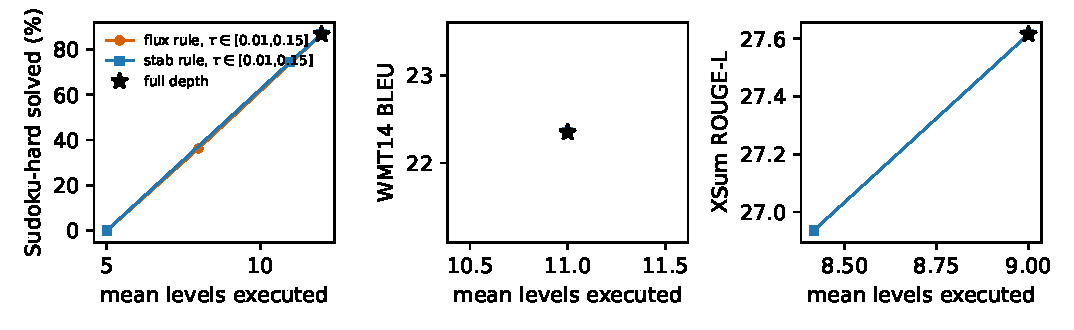
\includegraphics[width=\textwidth]{figs/fig_halt.pdf}
\caption{Quality versus mean executed levels for the flux and stability halting rules on uncorrected latents ($\tau\in\{0.01,\dots,0.15\}$, test items). Star: full depth. On WMT14 no setting halts; on XSum the stability rule at $\tau=0.15$ saves 0.6 levels on average at a cost of 0.7 ROUGE-L.}
\label{fig:halt}
\end{figure*}

\section{Additional figures and tables}
\label{app:extra_figs}
\begin{figure}[t]
\centering
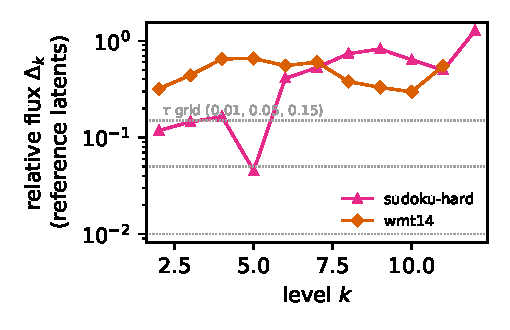
\includegraphics[width=\columnwidth]{figs/fig_flux.pdf}
\caption{Relative latent flux $\Delta_k$~\eqref{eq:flux} along reference trajectories of the released tokenizers (64 Sudoku-hard boards, 12 WMT14 sentences). Dotted lines mark the $\tau$ grid. The flux does not decay with $k$, which violates the premise of Proposition~\ref{prop:rd}.}
\label{fig:flux}
\end{figure}

\begin{figure}[t]\centering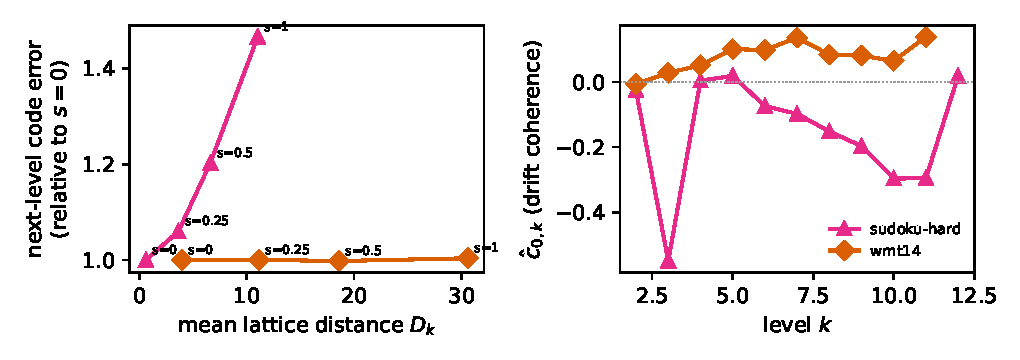
\includegraphics[width=0.85\linewidth]{figs/fig_offmanifold.pdf}
\caption{Measured constants of the revised Proposition~\ref{prop:contraction}. Left: next-level code error versus mean lattice distance when rollout states are revised by the in-loop corrector at step-size scale $s$ (seed-42 corrector). Right: per-level drift coherence $\hat c_{0,k}$ on greedy rollouts; negative values mean finer levels partially cancel accumulated drift.}\label{fig:offm}\end{figure}

\begin{figure}[t]
\centering
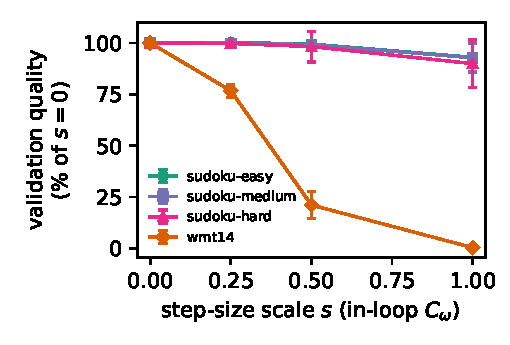
\includegraphics[width=\columnwidth]{figs/fig_dose.pdf}
\caption{Closed-loop validation quality of the in-loop corrector as a function of its step-size scale $s$ (relative to $s=0$, mean$\pm$std over five seeds; Sudoku: solve rate, WMT14: BLEU). Quality decreases monotonically with $s$; the effect is strongest for translation, where the generator is most sensitive to its input latent.}
\label{fig:dose}
\end{figure}

\begin{table*}[t]
\centering
\caption{Generator co-adaptation with 12{,}000 symmetry-augmented training boards (4 DAgger rounds of 1{,}000 fresh boards; checkpoint and corrector selected on 1{,}200 augmented validation boards; 1{,}500 held-out test boards; five seeds). Columns per arm: mean$\pm$std solve rate, one-sample $t$-test of seed means against NCM, smallest per-seed McNemar $p$, and the number of seeds for which validation selection kept the official generator.}
\label{tab:dagaug}
\small
\resizebox{\textwidth}{!}{\begin{tabular}{lc cccc cccc}
\toprule
& & \multicolumn{4}{c}{DAgger} & \multicolumn{4}{c}{DAgger + $C_\omega$}\\
\cmidrule(lr){3-6}\cmidrule(lr){7-10}
Task & NCM & solved & $t$-test $p$ & min.\ McN.\ $p$ & kept & solved & $t$-test $p$ & min.\ McN.\ $p$ & kept\\
\midrule
Sudoku-hard & 86.67 & 87.16$\pm$0.53 & 0.11 & 0.02 & 0/5 & 87.13$\pm$0.53 & 0.12 & 0.07 & 0/5 \\
Sudoku-medium & 96.00 & 95.71$\pm$0.27 & 0.07 & 0.29 & 2/5 & 95.92$\pm$0.17 & 0.36 & 0.59 & 1/5 \\
\bottomrule
\end{tabular}}
\end{table*}


